\documentclass[12pt]{article}
\usepackage[utf8]{inputenc}
\usepackage[russian]{babel}
\usepackage{graphicx}
\usepackage{placeins}
\graphicspath{{proteus/}{usart/}}

\title{Курс молодого бойца}
\author{Ушаков А. Е., Храмцов И. А., Кузнецов В. А.}
\date{\today}
\begin{document}



\maketitle


\newpage
\tableofcontents
\newpage

Этот мануал лежит на гитхабе $https://github.com/UshAle/new\_warrior\_course$.
если вы хотите дополнить или поправить его пишите на $ush.ale@yandex.ru$.
\section{Необходимый список программ}
\begin{itemize}
\item Atmel Studio 6
\newline Это весьма популярная среда программирования для контроллеров Atmel, предоставляется бесплатно.
\newline $http://www.atmel.com/tools/atmelstudio.aspx$
\item ChipProg Usb
\newline Среди оборудования ЛЭМФ есть программатор ChipProg40, способный программировать в параллельном режиме почти любой микроконтроллер.
Из-за его устройства наиболее удобно программировать микроконтролеры в DIP корпусе.
Сама программа устанавливается и запускается только при наличии подключенного к компьтеру программатора.
Иструкция к программе имеется на сайте разработчика.
\newline $http://www.phyton.ru/download/$
\item Sprint-Layout
\newline Простой, но в тоже время очень эффективный программный пакет для проектировки и ручной разводки печатных плат малой и средней сложности.
\newline $http://cxem.net/software/sprint\_layout.php$
\item Proteus (для моделирования всего и вся) Ссылку находить на торрентах:)
\end{itemize}
\section{Справочный материал}
\begin{itemize}
\item Atmega8a DataSheet
\newline Здесь можно найти всю информацию по распиновке контроллера, написания кода на C и ассемблере и прошивке.
\newline $http://www.atmel.com/images/atmel-8159-8-bit-avr-microcontroller-atmega8a\_datasheet.pdf$
\item Г. И. Донов "Применение микроконтроллеров"
\newline Эту книгу можно взять в библиотеке. Будет полезна тем, кто не хочет читать новый материал из даташита выше сразу на английском.
\item Информация по изготовлению печатных плат методом ЛУТ 
\newline $http://easyelectronics.ru/sozdanie-pechatnoj-platy-metodom-lazernogo-utyuga.html$
\item Руководство по разведению печатных плат с помощью программы SprintLayout 5.
\newline $http://easyelectronics.ru/sprint-layout-5-podrobnoe-rukovodstvo.html$
\item По оппонентной теории Геринга можно прочитать в дипломах А. Баранова и Е. Евдокимова. Они есть у А. И. Миланича.
\end{itemize}

\section{Оборудование ЛЭМФ}
В лабаратории есть некоторое количество печатных и макетных плат, которые мы здесь перечисляем.
\begin{itemize}
\item Макетная плата
\newline Такая же как на РТ лабах.
\item Несколько микроконтролеров Atmega8 в DIP корпусах.
\item Несколько rgb светодиодов.
\item Программатор ChipProg40
\item ISP переходник для программатора. Внимание, может пропадать контакт.
\item Изготовленные методом фрезерования 2 сторониие платы для монтажа схемы со светодиодом и ISP разъёмом.
\end{itemize}
\newpage
\section{Использование программ}
\subsection{Proteus}
После запуска Proteus(isis.exe) должно открыться окно как на рис.~\ref{p1} 
Чтобы выбрать микроконтроллер(или какой либо другой элемент) запустите окно Pick devices. рис.~\ref{p2}
Прошить микроконтроллер можно, выбрав соответствующий hex файл, в Edit component рис.~\ref{p3}  
\begin{figure}[h!]
\center{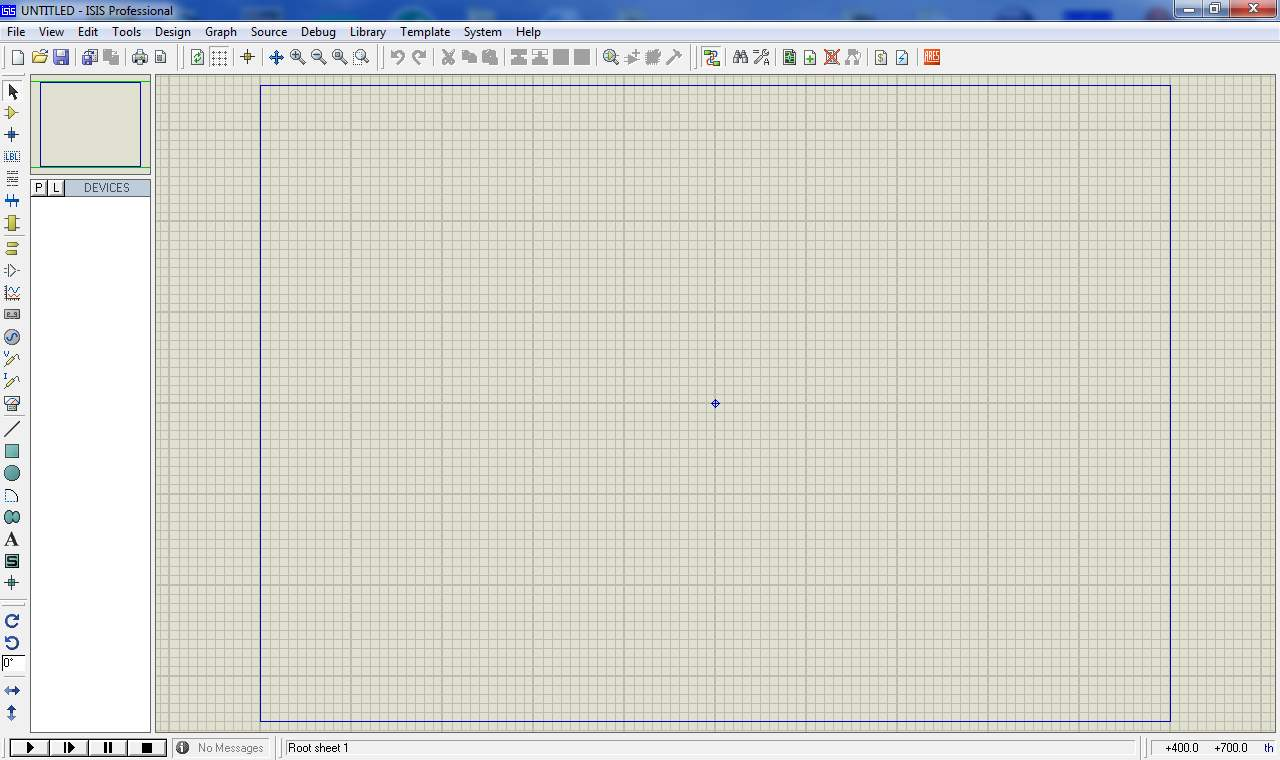
\includegraphics[width=1\linewidth]{1.jpg}}
\caption{Начальное окно Proteus}
\label{p1}
\end{figure}

\begin{figure}[h!]
\center{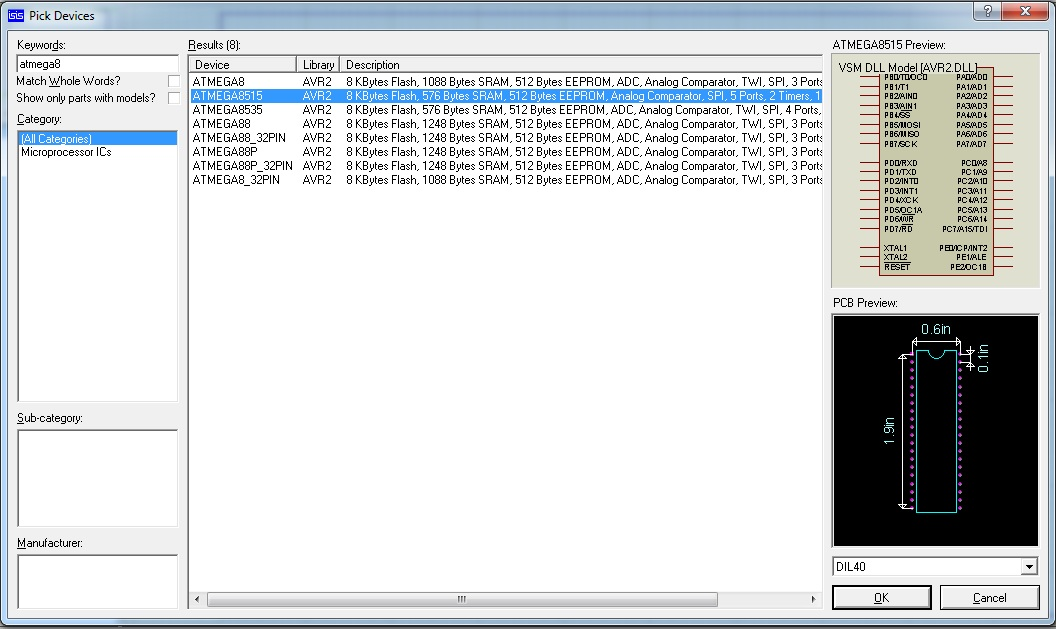
\includegraphics[width=1\linewidth]{2.jpg}}
\caption{Pick devices}
\label{p2}
\end{figure}

\begin{figure}[h!] 
\center{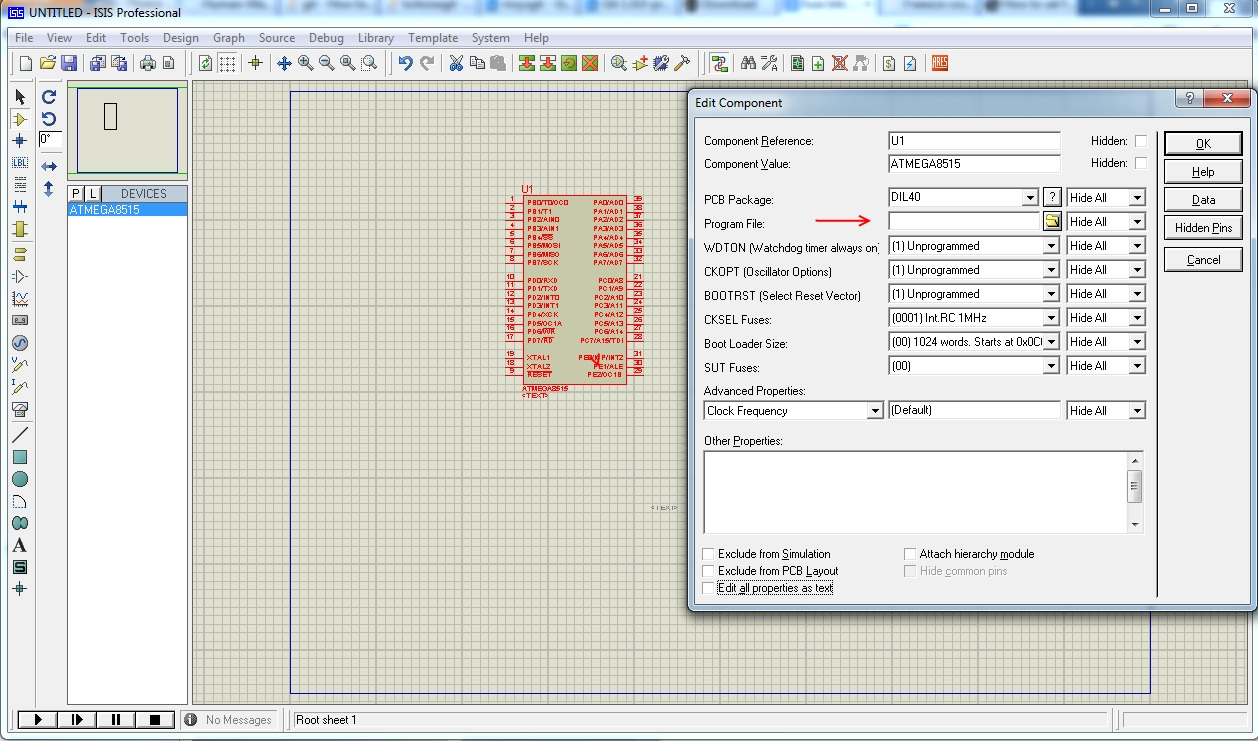
\includegraphics[width=1\linewidth]{3.jpg}}
\caption{Edit component}
\label{p3}
\end{figure}
Для моделирования usart в prodeus сделан компонент virual terminal. Важным неочевидным его свойством является то, что он может передавать определённую строку данных при запуске. Для этого 
в текстовом режиме редактирования компонента можно указать свойство text, в котором задать строку(рис ~\ref{vt}).
\begin{figure}[h!] 
\center{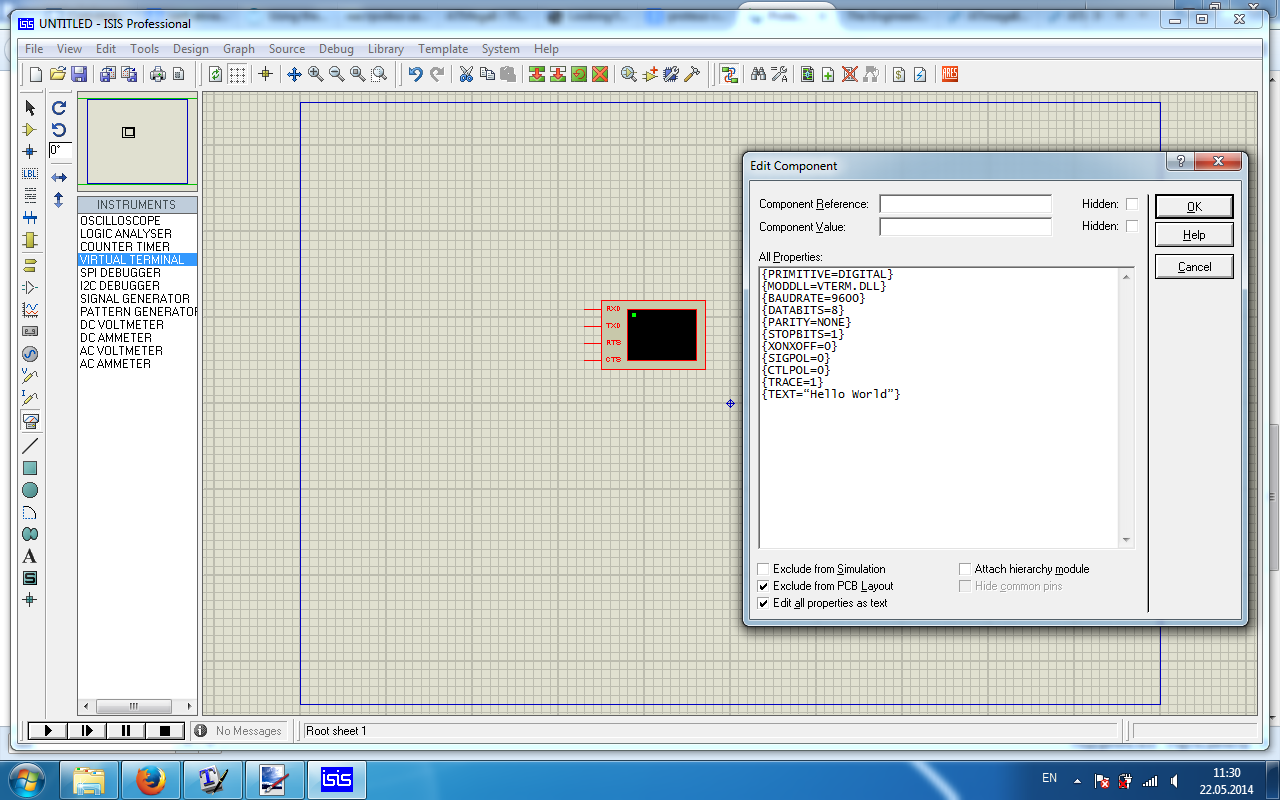
\includegraphics[width=1\linewidth]{vt.png}}
\caption{Virtual terminal}
\label{vt}
\end{figure}
\newpage
\subsection{Atmel Studio}

Запустив Atmel Studio, нужно создать проект для atmega8. Для этого нажмите NewProject GCC C Executable Project Atmega8. Теперь вы можете писать код на C для микроконтроллеров. Смотрите в примерах кода как использовать USART. 

\section{Примеры кода}

\subsection{Использование USART}
USART(Universal Asynchronous Receiver-Transmitter) нужен для того, чтобы предавать данные между элементми схемы.
\subsubsection{Описание}
Порт tx используется для передачи, rx для приёма. Соответственно соединяя элементы схемы нужно подключить rx к tx и наоборот.
\newline Скорость передачи USART измеряется в бодах (битах в секунду). Есть набор стандартных значений бодрейта: 300, 600, 1200, 2400, 4800, 9600, 19200, 38400, 57600, 115200, 230400, 460800, 921600 бод. Приёмник и передатчик должны быть настроены на одинаковый бодрейт, иначе будут происходить ошибки. 
\newline Опишем процесс передачи данных. Перед передачей напряжение на tx равно 1. Когда начинается передача напряжение перемещается в положение 0. Это является сигналом для приёмника, что передача началась. Затем следует несколько(обычно 8) поседовательных импульсов, которые передают ваши данные. После этого может следвать бит чётности,служащий для проверки данных и от одного до двух стопбитов. Процесс повторяется.
\begin{figure}[h!] 
\center{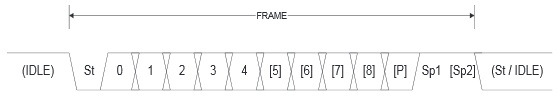
\includegraphics[width=1\linewidth]{usart1.jpg}}
\caption{USART}
\label{u1}
\end{figure}

\subsubsection{Код USART}
Самое сложное в USART - настроит бодрейт правильно. Для это нужно знать несколько вещей:
\begin{itemize}
\item Настроеить частоту микроконтроллера правильно
\item Использовать формулу для бодрейта из datasheet( рис.~\ref{eq1})
\item Знать параметры регистров UCSRB, UCSRC, UBRR, UCSRA, UDR
\end{itemize}
Почти работающий код usart.
\begin{verbatim}
/*
* AtMega8a.c
*
* Created: 24.10.2013 0:35:45
* Author: Igor
*/
#define __DELAY_BACKWARD_COMPATIBLE__
#include <avr/io.h>
#include <util/delay.h>
#include <avr/delay.h>
#define F_CPU 4000000UL//настройка частоты микроллера

int buf;
int ready;

void USART_Init(void)
{
UBRRH = 0;
UBRRL = 0;
//Назначение этих битов смотрите в datasheet
UCSRB = (1«RXEN)|(1«TXEN)|(1«RXCIE)|(0«TXCIE)|(0«UDRIE);
UCSRC = (1«URSEL)|(1«UCSZ1)|(1«UCSZ0);
buf=0;
ready=0;
Nget=0;
}

unsigned char USART_Receive( void )
{
/* Ждём данные для приёма */
while ( !(UCSRA & (1«RXC)) )
;
/* Возвращаем данные */
return UDR;
}

void USART_Transmit( unsigned char data )
{
/* Ждём когда буффер освободится */
while ( !( UCSRA & (1«UDRE)) )
;
/* Кладём туда данные */
UDR = data;
}

int main(void)
{

DDRB=0xFF; 
PORTB=0x00; 
USART_Init();//запускаем usart
while(1)
{
//передаём/принимаем
}
}
\end{verbatim}
\begin{figure}[h!]
\center{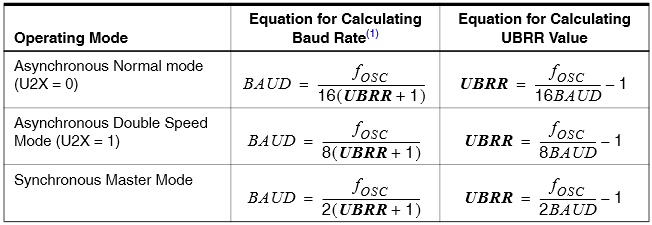
\includegraphics[width=1\linewidth]{eq.png}}
\caption{Формула для расчета бодрейта}
\label{eq1}
\end{figure}
\newpage
\subsection{Использование прерываний}

\end{document}
